\حصہ{تفرقی مساوات کے نظام}
لاپلاس بدل سے سادہ تفرقی مساوات کا نظام بھی حل کیا جا سکتا ہے۔ اس ترکیب کو چند مثالوں کی مدد سے سیکھتے ہیں۔آئیں سب سے پہلے مستقل عددی سر والے خطی، ایک درجی سادہ تفرقی مساوات [حصہ \حوالہ{حصہ_نظام_قالب} دیکھیں۔] کے نظام
\begin{gather}
\begin{aligned}\label{مساوات_لاپلاس_نظام_خطی_ایک_درجی_الف}
y_1'&=a_{11}y_1+a_{12}y_2+g_1(t)\\
y_2'&=a_{21}y_1+a_{22}y_2+g_2(t)
\end{aligned}
\end{gather}
پر غور کریں۔\عددی{\Laplace(y_1)=Y_1}، \عددی{\Laplace(y_2)=Y_2}، \عددی{\Laplace(g_1)=G_1} اور \عددی{\Laplace(g_2)=G_2} لکھتے ہوئے ضمنی نظام
\begin{align*}
sY_1-y_1(0)&=a_{11}Y_1+a_{12}Y_2+G_1(s)\\
sY_2-y_2(0)&=a_{21}Y_1+a_{22}Y_2+G_2(s)
\end{align*}
حاصل ہوتا ہے جس کو ترتیب دیتے ہوئے  درج ذیل لکھا جاسکتا ہے۔
 \begin{gather}
\begin{aligned}\label{مساوات_لاپلاس_نظام_خطی_ایک_درجی_ب}
(a_{11}-s)Y_1+a_{12}Y_2&=-y_1(0)-G_1(s)\\
a_{21}Y_1+(a_{22}-s)Y_2&=-y_2(0)-G_2(s)
\end{aligned}
\end{gather}
اس نظام کو الجبرائی طور پر حل کر کے \عددی{Y_1} اور \عددی{Y_2} حاصل ہوں گے جن سے \عددی{y_1=\Laplace^{-1}[Y_1(s)]} اور \عددی{y_2=\Laplace^{-1}[Y_2(s)]}  ملتا ہے جو نظام کا حل ہے۔

نظام \حوالہ{مساوات_لاپلاس_نظام_خطی_ایک_درجی_ب} اور نظام \حوالہ{مساوات_لاپلاس_نظام_خطی_ایک_درجی_ب} کو سمتیہ کی صورت میں لکھا جا سکتا ہے۔یوں \عددی{\bM{y}=[y_1\,\,\,y_2]^T}، \عددی{\bM{A}=[a_{jk}]}، \عددی{\bM{G}=[g_1\,\,\,g_2]^T}، \عددی{\bM{Y}=[Y_1\,\,\,Y_2]^T} اور \عددی{\bM{G}=[G_1\,\,\,G_2]^T} لکھتے ہوئے  درج ذیل لکھا جائے گا۔
\begin{align*}
\bM{y}'=\bM{A}\bM{y}+\bM{g} \quad \text{اور}\quad (\bM{A}-s\bM{I})\bM{y}=-\bM{y}(0)-\bM{G}
\end{align*}
%============================
\ابتدا{مثال}\شناخت{مثال_لاپلاس_ٹینکیوں_کا_نظام_الف}\quad مرکب تیار کرنے والا دو ٹینکیوں کا نظام\\
شکل \حوالہ{شکل_مثال_لاپلاس_ٹینکیوں_کا_نظام_الف} میں دو ٹینکیوں کا نظام دکھایا گیا ہے۔ابتدائی طور پر ٹینکی-الف میں دو سو لٹر \عددی{(\SI{200}{\litre})} خالص  پانی جبکہ ٹینکی-ب میں پچاس کلوگرام \عددی{(\SI{50}{\kilo\gram})} نمک ملا دو سو لٹر پانی پایا جاتا ہے۔نظام کے باہر سے ٹینکی-الف میں پانی کا داخلی بہاو چار لٹر فی منٹ ہے جس میں نمک کی شرح \عددی{\tfrac{1}{20}} کلوگرام فی لٹر  \عددی{(\SI{0.05}{\kilo\gram\per\litre})} ہے۔ٹینکیوں میں نمک کی مقدار بالمقابل وقت \عددی{y_1(t)} اور \عددی{y_2(t)} دریافت کریں۔
\begin{figure}
\centering
\begin{subfigure}{0.5\textwidth}
\centering
\begin{tikzpicture}
\draw(0,0) rectangle ++(-3/4*\x,\y);
\draw(\x,0) rectangle ++(3/4*\x,\y);
\draw(0,\y/4) rectangle ++(\x,\y/8);
\draw(0,3/4*\y) rectangle ++(\x,-\y/8);
\draw(-3/8*\x,\y/2)node[]{\RL{ٹینکی ب}};
\draw(\x+3/8*\x,\y/2)node[]{\RL{ٹینکی الف}};
\draw[latex-] (\x/4,\y/4+\y/16)--++(\x/2,0);
\draw[-latex] (\x/4,3/4*\y-\y/16)--++(\x/2,0);
\draw(\x/2,\y/4)node[below]{\RL{$6$ لٹر فی منٹ}};
\draw(\x/2,3/4*\y)node[above]{\RL{$2$ لٹر فی منٹ}};
\draw(-3/4*\x,1/8*\y) rectangle ++(-3/4*\x,\y/8);
\draw(\x+3/4*\x,7/8*\y) rectangle ++(3/4*\x,-\y/8);
\draw[-latex] (\x+3/4*\x+3/4*\x-\x/5,7/8*\y-\y/16)--++(-\x/3,0)node[pos=0.5,shift={(0,0.4)}]{\RL{$4$ لٹر فی منٹ}};
\draw[latex-] (-3/4*\x-3/4*\x+\x/5,1/8*\y+\y/16)--++(\x/3,0)node[pos=0.5,shift={(0,0.4)}]{\RL{$4$ لٹر فی منٹ}};
\end{tikzpicture}
\end{subfigure}
\begin{subfigure}{0.5\textwidth}
\centering
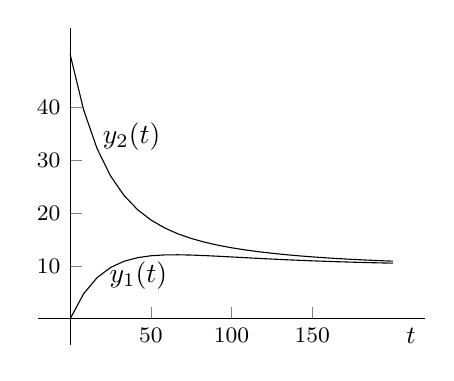
\begin{tikzpicture}
\begin{axis}[small,axis lines*=middle,xlabel={$t$},xlabel style={at={(current axis.right of origin)},anchor=north east},xtick={50,100,150},ytick={10,20,30,40}]
\addplot[domain=0:200]{10+6.56*e^(-0.0127*x)-16.56*e^(-0.0473*x)}node[pos=0.1,right]{$y_1(t)$};
\addplot[domain=0:200]{10+11.33*e^(-0.0127*x)+28.67*e^(-0.0473*x)}node[pos=0.1,right]{$y_2(t)$};
\end{axis}
\end{tikzpicture}
\end{subfigure}
\caption{مثال \حوالہ{مثال_لاپلاس_ٹینکیوں_کا_نظام_الف} میں ٹینکیوں کا نظام۔}
\label{شکل_مثال_لاپلاس_ٹینکیوں_کا_نظام_الف}
\end{figure}%

حل:نظام کا نمونہ درج ذیل مساوات سے لکھا جائے گا (حصہ \حوالہ{حصہ_نظام_قالب} دیکھیں)۔
\begin{align*}
\text{\RL{تبدیلی کی شرح}}=\text{\RL{داخلی بہاو فی منٹ}}-\text{\RL{خارجی بہاو فی منٹ}}
\end{align*}
یوں درج ذیل لکھا جا سکتا ہے جہاں ابتدائی معلومات \عددی{y_1(0)=0} اور \عددی{y_2(0)=50} ہیں۔
\begin{align*}
y_1'=-\frac{6}{200}y_1+\frac{2}{200}y_2+4(0.05)\quad \quad y_2'=\frac{6}{200}y_1-\frac{2}{200}y_2-\frac{4}{200}y_2
\end{align*}
اس طرح ضمنی نظام درج ذیل ہو گا۔
\begin{align*}
-(0.03+s)Y_1+0.01Y_2&=-\frac{0.2}{s}\\
0.03Y_1-(0.03+s)Y_2&=-50
\end{align*}
ضمنی نظام کے دو عدد ہمزاد مساوات کو الجبرائی طور پر حل کرتے ہوئے \عددی{Y_1} اور \عددی{Y_2} حاصل کرتے ہیں۔
\begin{align*}
Y_1&=\frac{3500s+30}{5000s^2+300s+3}=\frac{10}{s}+\frac{6.56}{s+0.0127}-\frac{16.56}{s+0.0473}\\
Y_2&=\frac{250000s^2+7500s+30}{5000s^2+300s+3}=\frac{10}{s}+\frac{11.33}{s+0.0127}+\frac{28.67}{s+0.0473}
\end{align*}
ان کا الٹ لاپلاس بدل لکھتے ہیں جو نظام کا حل ہے۔
\begin{align*}
y_1(t)&=10+6.56e^{-0.0127t}-16.56e^{-0.0473t}\\
y_2(t)&=10+11.33e^{-0.0127t}+28.67e^{-0.0473}
\end{align*}
%

\انتہا{مثال}
%================================
\ابتدا{مثال}\شناخت{مثال_لاپلاس_دور_دو_امالہ_الف}\quad برقی دور\\
برقی دور کو شکل \حوالہ{شکل_مثال_لاپلاس_دور_دو_امالہ_الف} میں دکھایا گیا ہے۔منبع کا دباو \عددی{v_m(t)} وقت \عددی{t=0} تا \عددی{t=0.5} سیکنڈ کے لئے \عددی{100} وولٹ ہے جبکہ بقایا اوقات اس کی قیمت صفر کے برابر ہے۔رو \عددی{i_1(t)} اور \عددی{i_2(t)} دریافت کریں۔ 
\begin{figure}
\centering
\begin{subfigure}{0.5\textwidth}
\centering
\begin{tikzpicture}
\draw(0,0) to [american voltage source,l={$v_m(t)$}]++(0,\y) to [inductor,l={$\SI{0.8}{\henry}$}]++(\x,0) to [resistor]++(0,-\y) to [resistor,l={$\SI{1.4}{\ohm}$}]++(-\x,0);
\draw(\x,0)node[above right]{$\SI{1}{\ohm}$};
\draw(\x,\y) to [short,*-]++(\x,0) to [inductor,l={$\SI{1}{\henry}$}]++(0,-\y) to [short,-*]++(-\x,0);
\draw[stealth-] ([shift={(-150:\x/4)}]\x/2,\y/2) arc (-150:150:\x/4);
\draw[stealth-] ([shift={(-150:\x/4)}]\x+\x/2,\y/2) arc (-150:150:\x/4);
\draw(\x/2,\y/2)node[]{$i_1$};
\draw(\x+\x/2,\y/2)node[]{$i_2$};
\end{tikzpicture}
\end{subfigure}%
\begin{subfigure}{0.5\textwidth}
\centering
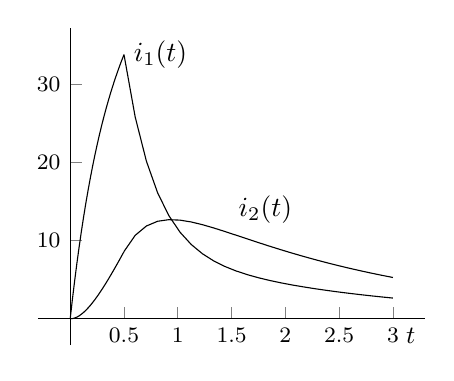
\begin{tikzpicture}
\begin{axis}[small,axis lines*=middle,xlabel={$t$},xlabel style={at={(current axis.right of origin)},anchor=north east}]
\addplot[domain=0:0.5]{500/7-125/3*e^(-1*x/2)-625/21*e^(-7*x/2)}node[right]{$i_1(t)$};
\addplot[domain=0:0.5]{500/7-250/3*e^(-1*x/2)+250/21*e^(-7*x/2)};
\addplot[domain=0.5:3]{-125/3*(1-e^(1/4))*e^(-x/2)-625/21*(1-e^(7/4))*e^(-7*x/2)};
\addplot[domain=0.5:3]{-250/3*(1-e^(1/4))*e^(-x/2)+250/21*(1-e^(7/4))*e^(-7*x/2)}node[pos=0.5,above right]{$i_2(t)$};
\end{axis}
\end{tikzpicture}
\end{subfigure}%
\caption{مثال \حوالہ{مثال_لاپلاس_دور_دو_امالہ_الف} کا دور اور اس کی برقی رو۔}
\label{شکل_مثال_لاپلاس_دور_دو_امالہ_الف}
\end{figure}

حل:کرخوف قانون دباو سے درج ذیل لکھا جا سکتا ہے۔
\begin{align*}
0.8i_1'+1(i_1-i_2)+1.4i_1&=100[1-u(t-1)]\\
1(i_2-i_1)+1i_2'&=0
\end{align*}
ابتدائی معلومات \عددی{i_1(0)=0} اور \عددی{i_2(0)=0} استعمال کرتے ہوئے مساوات \حوالہ{مساوات_لاپلاس_درجہ_اول_تفرق} اور منتقلی کے دوسرے مسئلے کی مدد سے ضمنی نظام حاصل کرتے ہیں
\begin{align*}
(s+3)I_1-1.25I_2&=\frac{125}{s}(1-e^{-\frac{s}{2}})\\
-I_1+(s+1)I_2&=0
\end{align*}
جس کا الجبرائی حل درج ذیل ہے۔
\begin{align*}
I_1&=\frac{125(s+1)}{s(s+\frac{1}{2})(s+\frac{7}{2})}(1-e^{-\frac{s}{2}})\\
I_2&=\frac{125}{s(s+\frac{1}{2})(s+\frac{7}{2})}(1-e^{-\frac{s}{2}})
\end{align*}
دائیں اطراف جزو \عددی{1-e^{-\tfrac{1}{2}}} کے علاوہ حصے کے جزوی کسری پھیلاو درج ذیل ہیں
\begin{align*}
\frac{500}{7s}-\frac{125}{3(s+\frac{1}{2})}-\frac{625}{21(s+\frac{7}{2})}\\
\frac{500}{7s}-\frac{250}{3(s+\frac{1}{2})}+\frac{250}{21(s+\frac{7}{2})}
\end{align*}
جن کا الٹ لاپلاس بدل \عددی{t=0} تا \عددی{t=\tfrac{1}{2}} کا حل دیتے ہیں۔ 
\begin{align*}
i_1(t)&=\frac{500}{7}-\frac{125}{3}e^{-\frac{1}{2}t}-\frac{625}{21}e^{-\frac{7}{2}t}\\
i_2(t)&=\frac{500}{7}-\frac{250}{3}e^{-\frac{1}{2}t}+\frac{250}{21}e^{-\frac{7}{2}t}\quad \quad (0\le t \le \frac{1}{2})
\end{align*}
منتقلی کے دوسرے مسئلے کے تحت \عددی{t<\tfrac{1}{2}} کے لئے حل  درج ذیل ہو گا۔رو کو شکل \حوالہ{شکل_مثال_لاپلاس_دور_دو_امالہ_الف} میں دکھایا گیا ہے۔
\begin{align*}
i_1(t)&=-\frac{125}{3}(1-e^{\frac{1}{4}})e^{-\frac{t}{2}}-\frac{625}{21}(1-e^{\frac{7}{4}})e^{-\frac{7}{2}t}\\
i_2(t)&=-\frac{250}{3}(1-e^{\frac{1}{4}})e^{-\frac{t}{2}}+\frac{250}{21}(1-e^{\frac{7}{4}})e^{-\frac{7}{2}t}\quad \quad (t>\frac{1}{2}) 
\end{align*}
کیا آپ بتلا سکتے ہیں کہ آخر کار دونوں رو صفر کیوں ہو گی؟ 
\انتہا{مثال}
%=================================

بلند درجی تفرقی مساوات کے نظام کو بھی اسی طرح لاپلاس بدل کی مدد سے حل کیا جاتا ہے۔ آئیں اسپرنگ اور کمیت کا ایک ایسا نظام حل کریں۔

%==========================
\ابتدا{مثال}\شناخت{مثال_لاپلاس_اسپرنگ_اور_کمیت_نظام_الف}
دو عدد کمیت اور تین عدد اسپرنگ کا نظام شکل \حوالہ{شکل_مثال_لاپلاس_اسپرنگ_اور_کمیت_نظام_الف} میں دکھایا گیا ہے۔قصری قوت صفر کے برابر ہے۔ ساکن حال سے نیچے کی جانب فاصلہ \عددی{y_1(t)} اور \عددی{y_2(t)} مثبت تصور کیا گیا ہے۔ابتدائی معلومات \عددی{y_1(0)=1}، \عددی{y_2(0)=1}، \عددی{y_1'(0)=\sqrt{3k}} اور \عددی{y_2'(0)=-\sqrt{3k}} ہیں۔مسئلہ حل کریں۔
\begin{figure}
\centering
\begin{subfigure}{0.4\textwidth}
\centering
\begin{tikzpicture}
\pgfmathsetmacro{\width}{0.9}
\pgfmathsetmacro{\height}{0.9}
\node[circle,fill=gray,inner sep=2.5mm] (b) at (0,0) {} ++(-0.32,0) node[left]{${m_1=1}$};
\node[circle,fill=gray,inner sep=2.5mm] (c) at (0,-2) {};
\draw[decorate,decoration={coil,aspect=0.3, segment length=1.7mm, amplitude=3mm}] (0,2) -- (b)node[pos=0.5,shift={(0.6,0)}]{$k$}; 
\fill [pattern = north east lines] (-1,2) rectangle (1,2.2);
\draw[thick] (-1,2) -- (1,2);
%
\draw(c)++(-0.32,0) node[left]{${m_2=1}$};
\draw[dashed] (0.5,0)--++(1,0);
\draw[dashed] (0.5,-2)--++(1,0);
\draw[-latex] (1,0)--++(0,-0.5)node[pos=0.5,right]{$y_1(t)$};
\draw[-latex] (1,-2)--++(0,-0.5)node[pos=0.5,right]{$y_2(t)$};
%
\draw[decorate,decoration={coil,aspect=0.3, segment length=1.7mm, amplitude=3mm}] (c) -- (b)node[pos=0.5,shift={(0.6,0)}]{$k$}; 
%
\draw[decorate,decoration={coil,aspect=0.3, segment length=1.7mm, amplitude=3mm}] (0,-4) -- (c)node[pos=0.5,shift={(0.6,0)}]{$k$}; 
\fill [pattern = north east lines] (-1,-4) rectangle (1,-4.2);
\draw[thick] (-1,-4) -- (1,-4);
\end{tikzpicture}
\end{subfigure}%
\begin{subfigure}{0.6\textwidth}
\centering
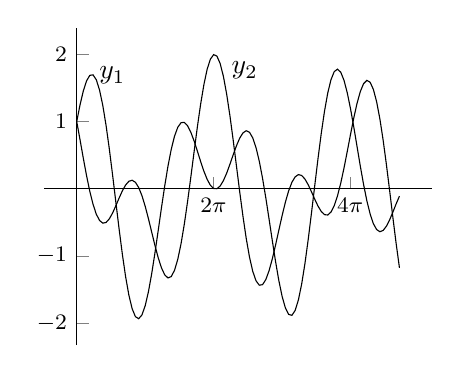
\begin{tikzpicture}
\begin{axis}[small,axis lines*=middle,xtick={360,720,1080},xticklabels={$2\pi$,$4\pi$,$6\pi$}]
\addplot[domain=0:850,samples=100]{cos(x)+sin(sqrt(3)*x)}node[pos=0.04,right]{$y_1$};
\addplot[domain=0:850,samples=100]{cos(x)-sin(sqrt(3)*x)}node[pos=0.45,right]{$y_2$};
\end{axis}
\end{tikzpicture}
\end{subfigure}%
\caption{اسپرنگ اور کمیت کا نظام (مثال \حوالہ{مثال_لاپلاس_اسپرنگ_اور_کمیت_نظام_الف})۔}
\label{شکل_مثال_لاپلاس_اسپرنگ_اور_کمیت_نظام_الف}
\end{figure}

حل:نیوٹن کا کلیہ کہتا ہے کہ کمیت ضرب اسراع برابر ہے قوت کے۔یوں بالائی اور نچلے کمیت کے لئے درج ذیل لکھا جا سکتا ہے۔
\begin{align*}
y_1''&=-ky_1+k(y_2-y_1)\\
y_2''&=-k(y_2-y_1)-ky_2
\end{align*} 
کمیت \عددی{m_1} پر بالائی اسپرنگ کی بنا \عددی{-ky_1} قوت عمل کرتا ہے جبکہ درمیانی اسپرنگ کی بنا اس پر \عددی{k(y_2-y_1)} قوت عمل کرتا ہے۔درمیانی اسپرنگ کی لمبائی میں کل اضافہ \عددی{y_2-y_1} کے برابر ہے۔کمیت \عددی{m_2} پر درمیانی اسپرنگ کی بنا \عددی{-k(y_2-y_1)} قوت عمل کرتا ہے  جبکہ نچلی اسپرنگ کی بنا اس پر \عددی{-ky_2} قوت عمل کرتا ہے۔ 

\عددی{\Laplace(y_1)=Y_1} اور \عددی{\Laplace(y_2)=Y_2} لکھتے ہوئے ابتدائی معلومات استعمال کرتے ہوئے مساوات \حوالہ{مساوات_لاپلاس_درجہ_دوم_تفرق} کی مدد سے  ضمنی مساوات لکھتے ہیں
\begin{align*}
s^2Y_1-s-\sqrt{3k}&=-kY_1+k(Y_2-Y_1)\\
s^2Y_2-s+\sqrt{3k}&=-k(Y_2-Y_1)-kY_2
\end{align*}
جن کو ترتیب دیتے ہوئے درج ذیل لکھا جا سکتا ہے۔
\begin{align*}
(s^2+2k)Y_1-kY_2&=s+\sqrt{3k}\\
-kY_1+(s^2+2k)Y_2&=s-\sqrt{3k}
\end{align*}
ان ہمزاد مساوات کا الجبرائی حل لکھتے ہیں۔
\begin{align*}
Y_1&=\frac{(s+\sqrt{3k})(s^2+2k)+k(s-\sqrt{3k})}{(s^2+2k)^2-k^2}=\frac{s}{s^2+k}+\frac{\sqrt{3k}}{s^2+3k}\\
Y_2&=\frac{(s-\sqrt{3k})(s^2+2k)+k(s+\sqrt{3k})}{(s^2+2k)^2-k^2}=\frac{s}{s^2+k}-\frac{\sqrt{3k}}{s^2+3k}
\end{align*}
الٹ لاپلاس بدل لیتے ہوئے حل حاصل کرتے ہیں
\begin{align*}
y_1(t)&=\cos \sqrt{k}t+\sin{\sqrt{3k}t}\\
y_2(t)&=\cos \sqrt{k}t-\sin{\sqrt{3k}t}
\end{align*}
جس کو شکل \حوالہ{شکل_مثال_لاپلاس_اسپرنگ_اور_کمیت_نظام_الف} میں دکھایا گیا ہے۔ آپ دیکھ سکتے ہیں کہ حرکت دو ہارمونی ارتعاش کا مجموعہ ہے۔

\انتہا{مثال}
%============================  

\حصہء{سوالات}

